\documentclass[12pt,letterpaper]{article}
\usepackage{fullpage}
\usepackage[top=2cm, bottom=4.5cm, left=2.5cm, right=2.5cm]{geometry}
\usepackage{amsmath,amsthm,amsfonts,amssymb,amscd}
\usepackage{lastpage}
\usepackage{enumerate}
\usepackage{fancyhdr}
\usepackage{mathrsfs}
\usepackage{xcolor}
\usepackage{fancyvrb}
\usepackage{graphicx}
\usepackage{listings}
\usepackage{float}
\usepackage{hyperref}
\usepackage{tikz}
\usepackage{relsize}
\usepackage{fancyvrb}
\usepackage{multirow}
\usepackage{booktabs}
\usepackage{import}
\usetikzlibrary{shapes.geometric,fit}

\hypersetup{%
  colorlinks=true,
  linkcolor=blue,
  linkbordercolor={0 0 1}
}

\setlength{\parindent}{0.0in}
\setlength{\parskip}{0.05in}

\theoremstyle{definition}
\newtheorem*{statement}{Statement}
\newtheorem*{claim}{Claim}
\newtheorem*{theorem}{Theorem}
\newtheorem*{lemma}{Lemma}

\newcommand{\contra}{\Rightarrow\!\Leftarrow}
\newcommand{\R}{\mathbb{R}}
\newcommand{\F}{\mathbb{F}}
\newcommand{\Z}{\mathbb{Z}}
\newcommand{\Zeq}{\mathbb{Z}_{\geq 0}}
\newcommand{\Zg}{\mathbb{Z}_{>0}}
\newcommand{\Req}{\mathbb{R}_{\geq 0}}
\newcommand{\Rg}{\mathbb{R}_{>0}}
\newcommand{\N}{\mathbb{N}}
\newcommand{\Q}{\mathbb{Q}}
\newcommand{\C}{\mathbb{C}}
\DeclareMathOperator{\Cov}{Cov}
\DeclareMathOperator{\Var}{Var}

\newcommand{\incfig}[1] {%
    \import{./figures/}{#1.pdf_tex}
}

\graphicspath{ {./figures/} }

\title{ECON 3412 HW 8}
\author{David Chen, dc3451}

\begin{document}

\maketitle

\section*{Problem 1}
\subsection*{a}

$(y_{1} - bx_{1})^{2} = (2 - b)^{2}$ is in blue.

\begin{figure}[H]
  \centering
  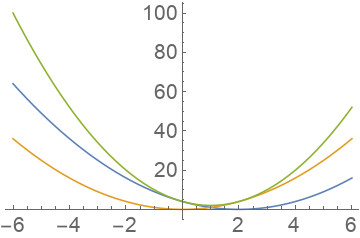
\includegraphics[width=8cm]{plot1.png}
\end{figure}

\subsection*{b}

This follows immediately from the fact that the blue (non-negative) curve in a vanishes at $b = 2$.

\subsection*{c}

This is given by the yellow curve above.

\subsection*{d}

This is given by the green curve above.

\subsection*{e}

The desired criteria $(2 - b)^{2} + b^{2}$ is minimized at $b = 1$, since the derivative is $-2(2 - b) + 2b$ which vanishes at $b = 1$, so $\hat{\beta}_{ridge} = 1$.

\subsection*{f}

\begin{figure}[H]
  \centering
  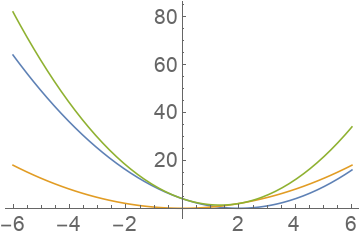
\includegraphics[width=8cm]{plot2.png}
\end{figure}

The penalty term is given by the yellow curve above, and the penalized term is green. We have that the sum is minimal when $-2(2 - b) + b = 0$, so $\hat{\beta}_{ridge} = \frac{4}{3}$.

\subsection*{g}

\begin{figure}[H]
  \centering
  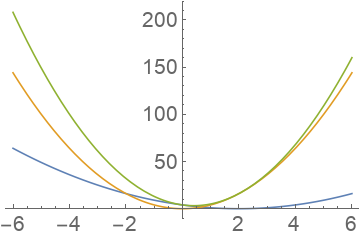
\includegraphics[width=8cm]{plot3.png}
\end{figure}

The penalty term is given by the yellow curve above, and the penalized term is green. We have that the sum is minimal when $-2(2 - b) + 8b = 0$, so $\hat{\beta}_{ridge} = \frac{2}{5}$.

\subsection*{h}

Algebraically, in the expression for the ridge estimator
\[
  \hat{\beta}_{ridge} = \frac{\hat{\beta}}{1 + \lambda_{ridge}/\sum x_{i}^{2}}
\]
we see that this is monotonically decreasing in $\lambda$ since the denominator is monotonically increasing in $\lambda$.

Morally, we see that the penalty term is large for larger values of $b$, and for larger $\lambda$ the penalty term is relatively more important for larger values of $\lambda$, so the minimizing quantity for $b$ is closer to $b = 0$, which minimizes the penalty term.

\subsection*{i, j}

The penalty term is in yellow and the sum in green.

\begin{figure}[H]
  \centering
  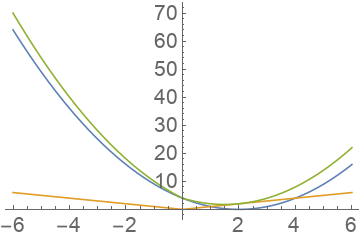
\includegraphics[width=8cm]{plot4.png}
\end{figure}

\subsection*{k}

We compute the derivative on the positive half-line to be $\lambda - 2(2 - b) = 2b - (4 - \lambda)$, so we have that the adjusted estimator is $\beta = \frac{4 - \lambda}{2}$ when this quantity is non-negative. In the case that it is negative, the function is increasing on the positive half-line and clearly decreasing on the negative half, so the estimator is $\beta = 0$.

In this case, $\beta_{lasso} = \frac{3}{2}$.

\subsection*{l}

The colorscheme is the same as above. $\beta_{lasso} = \frac{7}{4}$.

\begin{figure}[H]
  \centering
  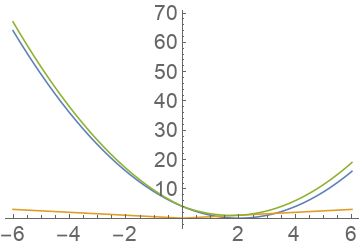
\includegraphics[width=8cm]{plot5.png}
\end{figure}

\subsection*{m}

The colorscheme is the same as above. $\beta_{lasso} = 0$, since the penalized sum increases on $b > 0$.

\begin{figure}[H]
  \centering
  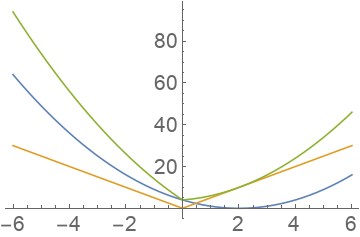
\includegraphics[width=8cm]{plot6.png}
\end{figure}

\subsection*{n}

The reasoning is more or less the same as the one for ridge; the penalty term increases for large $\beta$, and grows in importance with $\lambda_{lasso}$, so we get that for larger $\lambda$, the optimal $\beta$ minimizes the penalty term so $\beta$ shrinks.

Algebraically, we have that $\beta = \max\{0, (4 - \lambda)/2\}$ is clearly decreasing (up to $\lambda = 4$) in $\lambda$.

\section*{Problem 2}

\subsection*{a}

\begin{Verbatim}[fontsize=\small]
gen_lags <- function(df, var, lags) {
  data <- eval(substitute(var), df)
  for (i in 1:lags) {
    data <- append(data, NA, after = 0)[1:length(data)]
    names <- append(colnames(df), paste(deparse(substitute(var)), "lag", i, sep = ""))
    df <- cbind(df, data)
    colnames(df) <- names
  }
  return (df)
}

> growth <- read_dta("growth.dta")
> growth <- gen_lags(growth, growth, 4)
> growth <- gen_lags(growth, per_ip, 4)
> growth.ar1 <- lm(growth ~ growthlag1, data = growth)
> coeftest(growth.ar1, vcovCL)

t test of coefficients:

            Estimate Std. Error t value  Pr(>|t|)
(Intercept) 0.464434   0.144178  3.2213  0.001424 **
growthlag1  0.851983   0.036508 23.3372 < 2.2e-16 ***
---
Signif. codes:  0 ‘***’ 0.001 ‘**’ 0.01 ‘*’ 0.05 ‘.’ 0.1 ‘ ’ 1
\end{Verbatim}

\subsection*{b}

In Q1 2020, the growth was 0.3 (I assume 0.3\%? Not sure if it is annualized growth, but it seems like it), so we get that the model predicts $0.4644 + 0.3(0.8520) = 0.72\%$ growth in real GDP in Q2 2020 (I wish).

\subsection*{c}

\begin{Verbatim}[fontsize=\small]
> growth.ar4 <- lm(growth ~ growthlag1 + growthlag2 +
+                    growthlag3 + growthlag4,
+                  data = growth)
> coeftest(growth.ar4, vcovCL)

t test of coefficients:

             Estimate Std. Error t value  Pr(>|t|)
(Intercept)  0.843895   0.147057  5.7386 2.477e-08 ***
growthlag1   1.180945   0.072382 16.3155 < 2.2e-16 ***
growthlag2  -0.268231   0.112064 -2.3936   0.01734 *
growthlag3  -0.156513   0.108131 -1.4474   0.14889
growthlag4  -0.023423   0.067842 -0.3453   0.73016
---
Signif. codes:  0 ‘***’ 0.001 ‘**’ 0.01 ‘*’ 0.05 ‘.’ 0.1 ‘ ’ 1
\end{Verbatim}

\subsection*{d}

In Q2-4 2019, the growth was 2.3, 2.1, 2.3, so the model predicts growth of $0.843895 + 1.180945(0.3) - 0.268231(2.3)  - 0.156513(2.1) - 0.023423(2.3) = 0.198\%$ real GDP growth.

\subsection*{e}

\begin{Verbatim}[fontsize=\small]
> growth.adl11 <- lm(growth ~ growthlag1 + per_iplag1,
+                    data = growth)
> coeftest(growth.adl11, vcovCL)

t test of coefficients:

              Estimate Std. Error t value  Pr(>|t|)
(Intercept)  0.4564177  0.1440373  3.1687  0.001698 **
growthlag1   0.8578137  0.0469042 18.2886 < 2.2e-16 ***
per_iplag1  -0.0080086  0.0361859 -0.2213  0.825004
---
Signif. codes:  0 ‘***’ 0.001 ‘**’ 0.01 ‘*’ 0.05 ‘.’ 0.1 ‘ ’ 1
\end{Verbatim}

\subsection*{f}

The $per\_ip$ in Q1 2020 was $-21299$, so we get a prediction of $0.4564177 + 0.8578137(0.3) - 0.0080086(-2.1299) = 0.7308\%$ real GDP growth.

\subsection*{g}

\begin{Verbatim}[fontsize=\small]
> growth.adl44 <- lm(growth ~ growthlag1 + growthlag2 + growthlag3 + growthlag4 +
+                      per_iplag1 + per_iplag2 + per_iplag3 + per_iplag4,
+                    data = growth)
> coeftest(growth.adl44, vcovCL)

t test of coefficients:

             Estimate Std. Error t value  Pr(>|t|)
(Intercept)  0.853976   0.140510  6.0777 4.039e-09 ***
growthlag1   1.031432   0.079041 13.0493 < 2.2e-16 ***
growthlag2  -0.078673   0.116970 -0.6726 0.5017675
growthlag3  -0.184126   0.116740 -1.5772 0.1158876
growthlag4  -0.064528   0.078673 -0.8202 0.4128111
per_iplag1   0.344955   0.082090  4.2021 3.574e-05 ***
per_iplag2  -0.519814   0.138186 -3.7617 0.0002061 ***
per_iplag3   0.185744   0.142486  1.3036 0.1934581
per_iplag4   0.050592   0.078605  0.6436 0.5203524
---
Signif. codes:  0 ‘***’ 0.001 ‘**’ 0.01 ‘*’ 0.05 ‘.’ 0.1 ‘ ’ 1
\end{Verbatim}

\subsection*{h}

\begin{Verbatim}[fontsize=\small]
> linearHypothesis(growth.adl44, c("per_iplag1 = 0", "per_iplag2 = 0",
+                                  "per_iplag3 = 0", "per_iplag4 = 0"),
+                  vcov = vcovHC(growth.adl44, "HC1"))
+
Linear hypothesis test

Hypothesis:
per_iplag1 = 0
per_iplag2 = 0
per_iplag3 = 0
per_iplag4 = 0

Model 1: restricted model
Model 2: growth ~ growthlag1 + growthlag2 + growthlag3 + growthlag4 +
    per_iplag1 + per_iplag2 + per_iplag3 + per_iplag4

Note: Coefficient covariance matrix supplied.

  Res.Df Df      F    Pr(>F)
1    280
2    276  4 5.4069 0.0003319 ***
---
Signif. codes:  0 ‘***’ 0.001 ‘**’ 0.01 ‘*’ 0.05 ‘.’ 0.1 ‘ ’ 1
\end{Verbatim}

The Granger ``causality'' test is really just checking if the lagged regressors are jointly significant. In this case, we have that $F = 5.4$ and $p < 0.001$, so there are jointly significant and thus changes in industrial production do ``cause'' growth.

\section*{Problem 3}
\subsection*{a}

The problem set is unclear w/ parentheses, but the data set contains descriptions that make it seem like this question is asking only for regressing $gprice = \beta_{0} + \beta_{1}gwage + u$, and we don't have to generate the growth rate ourselves.

\begin{Verbatim}[fontsize=\small]
> wage.ols <- lm(gprice ~ gwage, data = wage)
> coeftest(wage.ols, vcovCL)

t test of coefficients:

              Estimate Std. Error t value  Pr(>|t|)
(Intercept) 0.00382414 0.00026051 14.6795 < 2.2e-16 ***
gwage       0.16580689 0.03779605  4.3869 1.624e-05 ***
---
Signif. codes:  0 ‘***’ 0.001 ‘**’ 0.01 ‘*’ 0.05 ‘.’ 0.1 ‘ ’ 1
\end{Verbatim}

Interpreting, we see that a unit increase in the growth of wages (that is, a 1\% increase) results in an (statistically significant, $p < 10^{-4}$) increase, on average, in the growth rate of general prices by $0.1658\%$, so the faster wages grow, the faster prices grow.

\subsection*{b}

The assumptions of the distributed lag model are that $X$ must be exogenous, such that $E(u \mid X_{t}, X_{t-1}, \dots) = 0$, that the distributions of $Y, X$ are stationary in time, such that the situations of $Y, X$ are fixed throughout time, and $(Y_{t}, X_{t})$ and $(Y_{t-i}, X_{t-i})$ are independent as $i$ becomes large. Furthermore, there cannot be perfect multicolinearity and we must have eight finite moments (that is, in some sense the tails cannot be too fat).

Standard errors, since we have autocorrelation, must be computed as HAC SE's, and we can do this with the Newey-West estimator (note that the \verb|R| implmentation may have slightly different default implementations from STATA, so the numbers could be off by a little). Truncation parameter is chosen by the default implementation, which is (from the documentation) I think the usual $0.75T^{1/3}$. The reason we need HAC SE's is that the earlier assumptions do not imply that wages and the errors are i.i.d; in fact, there is probably serial correlation, since prices being lower/higher than predicted by the model might either cause or be a sign of other economic issues that affect future prices being lower/higher, for example continued low wages might destablize some economy and wildly change the error of the model, so we get serial correlation.
\begin{Verbatim}[fontsize=\small]
> wage.tsols <- lm(gprice ~ gwage + gwage_1 + gwage_2 + gwage_3 + gwage_4 +
+                    gwage_5 + gwage_6 + gwage_7 + gwage_8 + gwage_9 +
+                    gwage_10 + gwage_11 + gwage_12,
+                  data = wage)
+ coeftest(wage.tsols, vcov = NeweyWest(wage.tsols))
+
t test of coefficients:

               Estimate  Std. Error t value  Pr(>|t|)
(Intercept) -0.00092960  0.00090528 -1.0269 0.3054430
gwage        0.11904158  0.06216537  1.9149 0.0566044 .
gwage_1      0.09721735  0.03602250  2.6988 0.0074168 **
gwage_2      0.03995177  0.03805352  1.0499 0.2947503
gwage_3      0.03826524  0.03648177  1.0489 0.2952081
gwage_4      0.08133615  0.03412153  2.3837 0.0178596 *
gwage_5      0.10685195  0.03574420  2.9894 0.0030646 **
gwage_6      0.09497313  0.04317740  2.1996 0.0287189 *
gwage_7      0.10379216  0.03750827  2.7672 0.0060621 **
gwage_8      0.10256285  0.03986800  2.5726 0.0106527 *
gwage_9      0.15850787  0.04533934  3.4960 0.0005554 ***
gwage_10     0.11044122  0.04542245  2.4314 0.0157184 *
gwage_11     0.10332057  0.04142016  2.4945 0.0132390 *
gwage_12     0.01565751  0.04868848  0.3216 0.7480261
---
Signif. codes:  0 ‘***’ 0.001 ‘**’ 0.01 ‘*’ 0.05 ‘.’ 0.1 ‘ ’ 1
\end{Verbatim}

\begin{figure}[H]
  \centering
  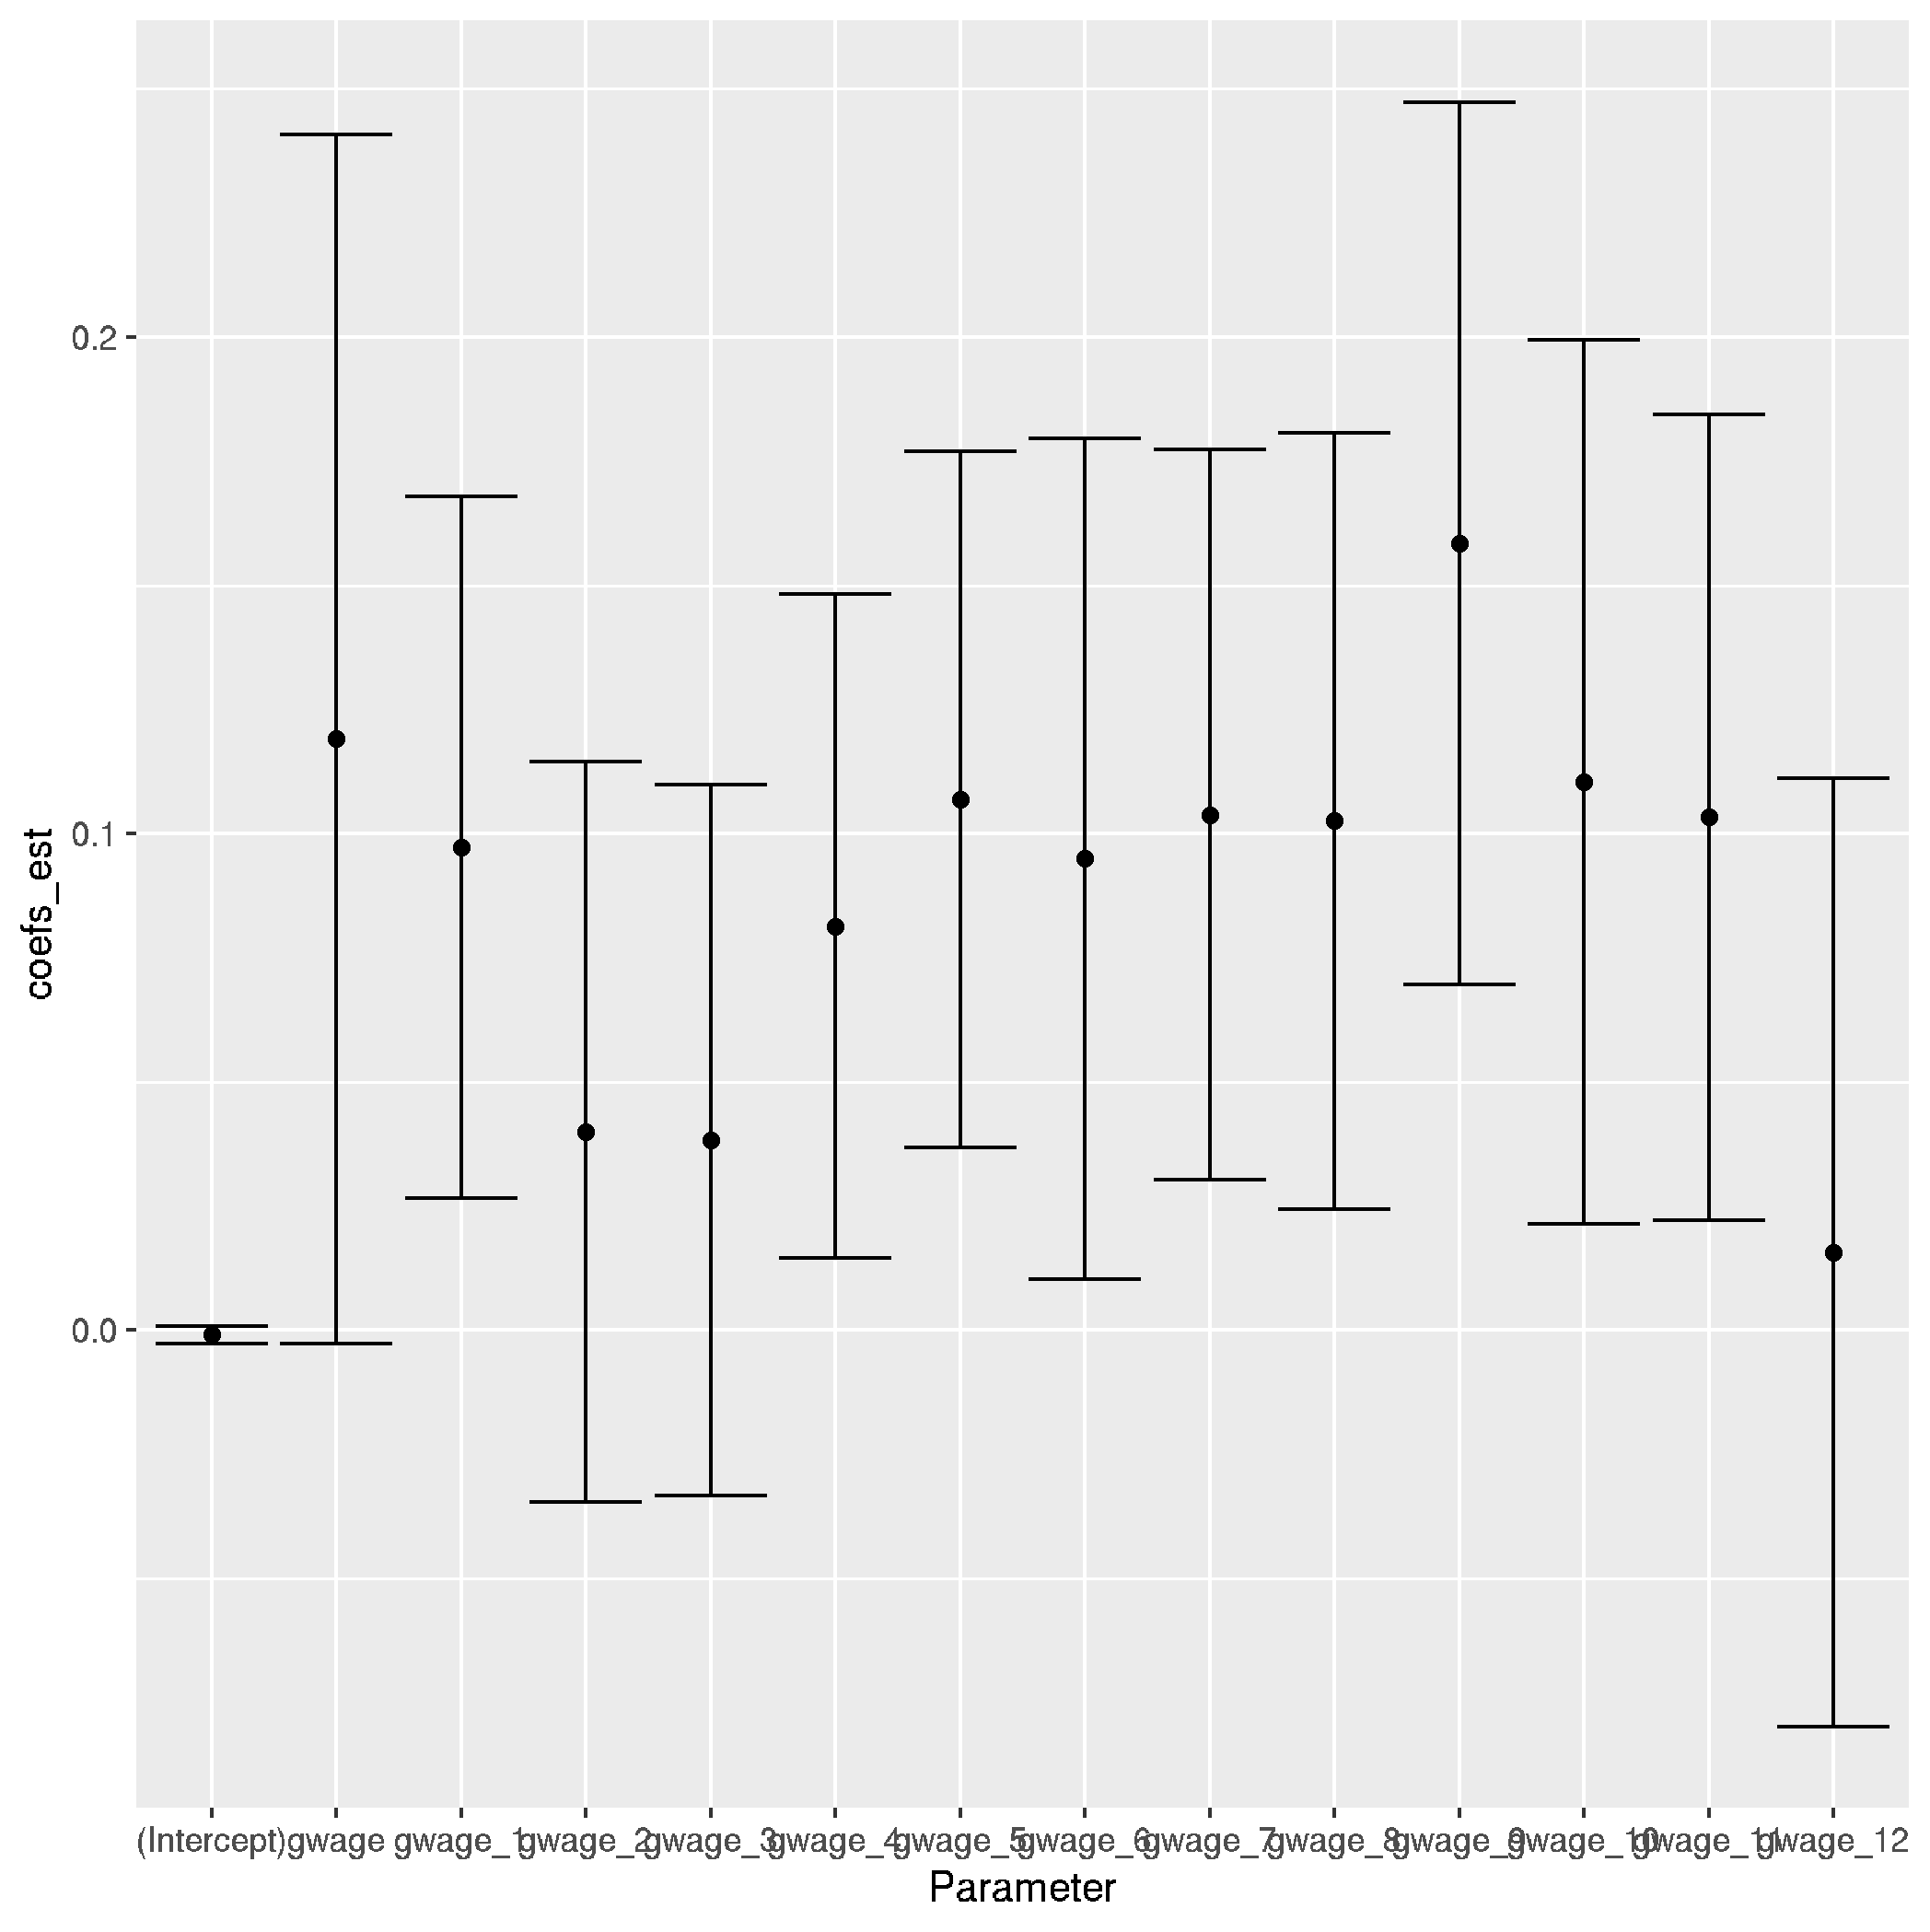
\includegraphics[width=10cm]{plot.png}
\end{figure}

We have

\subsection*{c}

\begin{Verbatim}[fontsize=\small]
> wage.tscumols <- lm(gprice ~ delta_0 + delta_1 + delta_2 + delta_3 + delta_4 +
+                       delta_5 + delta_6 + delta_7 + delta_8 + delta_9 +
+                       delta_10 + delta_11 + gwage_12,
+                     data = wage)
> coeftest(wage.tscumols, vcov = NeweyWest(wage.tscumols))
t test of coefficients:

               Estimate  Std. Error t value  Pr(>|t|)
(Intercept) -0.00092960  0.00090528 -1.0269 0.3054430
delta_0      0.11904158  0.06216537  1.9149 0.0566044 .
delta_1      0.21625893  0.07977154  2.7110 0.0071571 **
delta_2      0.25621070  0.10371451  2.4703 0.0141430 *
delta_3      0.29447594  0.13189240  2.2327 0.0264238 *
delta_4      0.37581209  0.14236261  2.6398 0.0087982 **
delta_5      0.48266405  0.14558445  3.3154 0.0010462 **
delta_6      0.57763718  0.15666632  3.6871 0.0002764 ***
delta_7      0.68142934  0.16392939  4.1568 4.389e-05 ***
delta_8      0.78399219  0.17236983  4.5483 8.314e-06 ***
delta_9      0.94250006  0.17869547  5.2743 2.814e-07 ***
delta_10     1.05294127  0.18860573  5.5828 5.968e-08 ***
delta_11     1.15626184  0.20032890  5.7718 2.235e-08 ***
gwage_12     1.17191935  0.20432092  5.7357 2.701e-08 ***
---
Signif. codes:  0 ‘***’ 0.001 ‘**’ 0.01 ‘*’ 0.05 ‘.’ 0.1 ‘ ’ 1
\end{Verbatim}

The cumulative multiplier is about 1 starting at the 10th lagged period, so about 10 months for wages to be fully incorporated into price changes.

\end{document}
% LocalWords:  NetID fancyplain LocalWords colorlinks linkcolor linkbordercolor
